% \documentclass[]{article}
\documentclass[fontset=overleaf,12pt]{ctexart}
\usepackage{fontspec}
% \usepackage{xeCJK}
\usepackage[a4paper,top=2cm,bottom=2cm,left=3cm,right=3cm,marginparwidth=1.75cm]{geometry}
\usepackage{lettrine}

\usepackage{amsmath}
\usepackage{graphicx}
\usepackage[colorlinks=true, allcolors=blue]{hyperref}


% 设置中文字体为宋体
% \setCJKmainfont{SimSun}
% \setCJKmainfont{KaiTi}
\usepackage{booktabs}
\usepackage{multirow}
\usepackage{tabularx}

% 设置英文字体为New Times

\setmainfont{Times New Roman}



\title{Artificial Generate Intelligence(AGI){\songti 行业分析}}
\author{\heiti 张桐林}
\date{}


% \author{Tony Zhang}
% \date{May 2023}

\begin{document}

\maketitle



\begin{figure}[htbp]
    \centering
    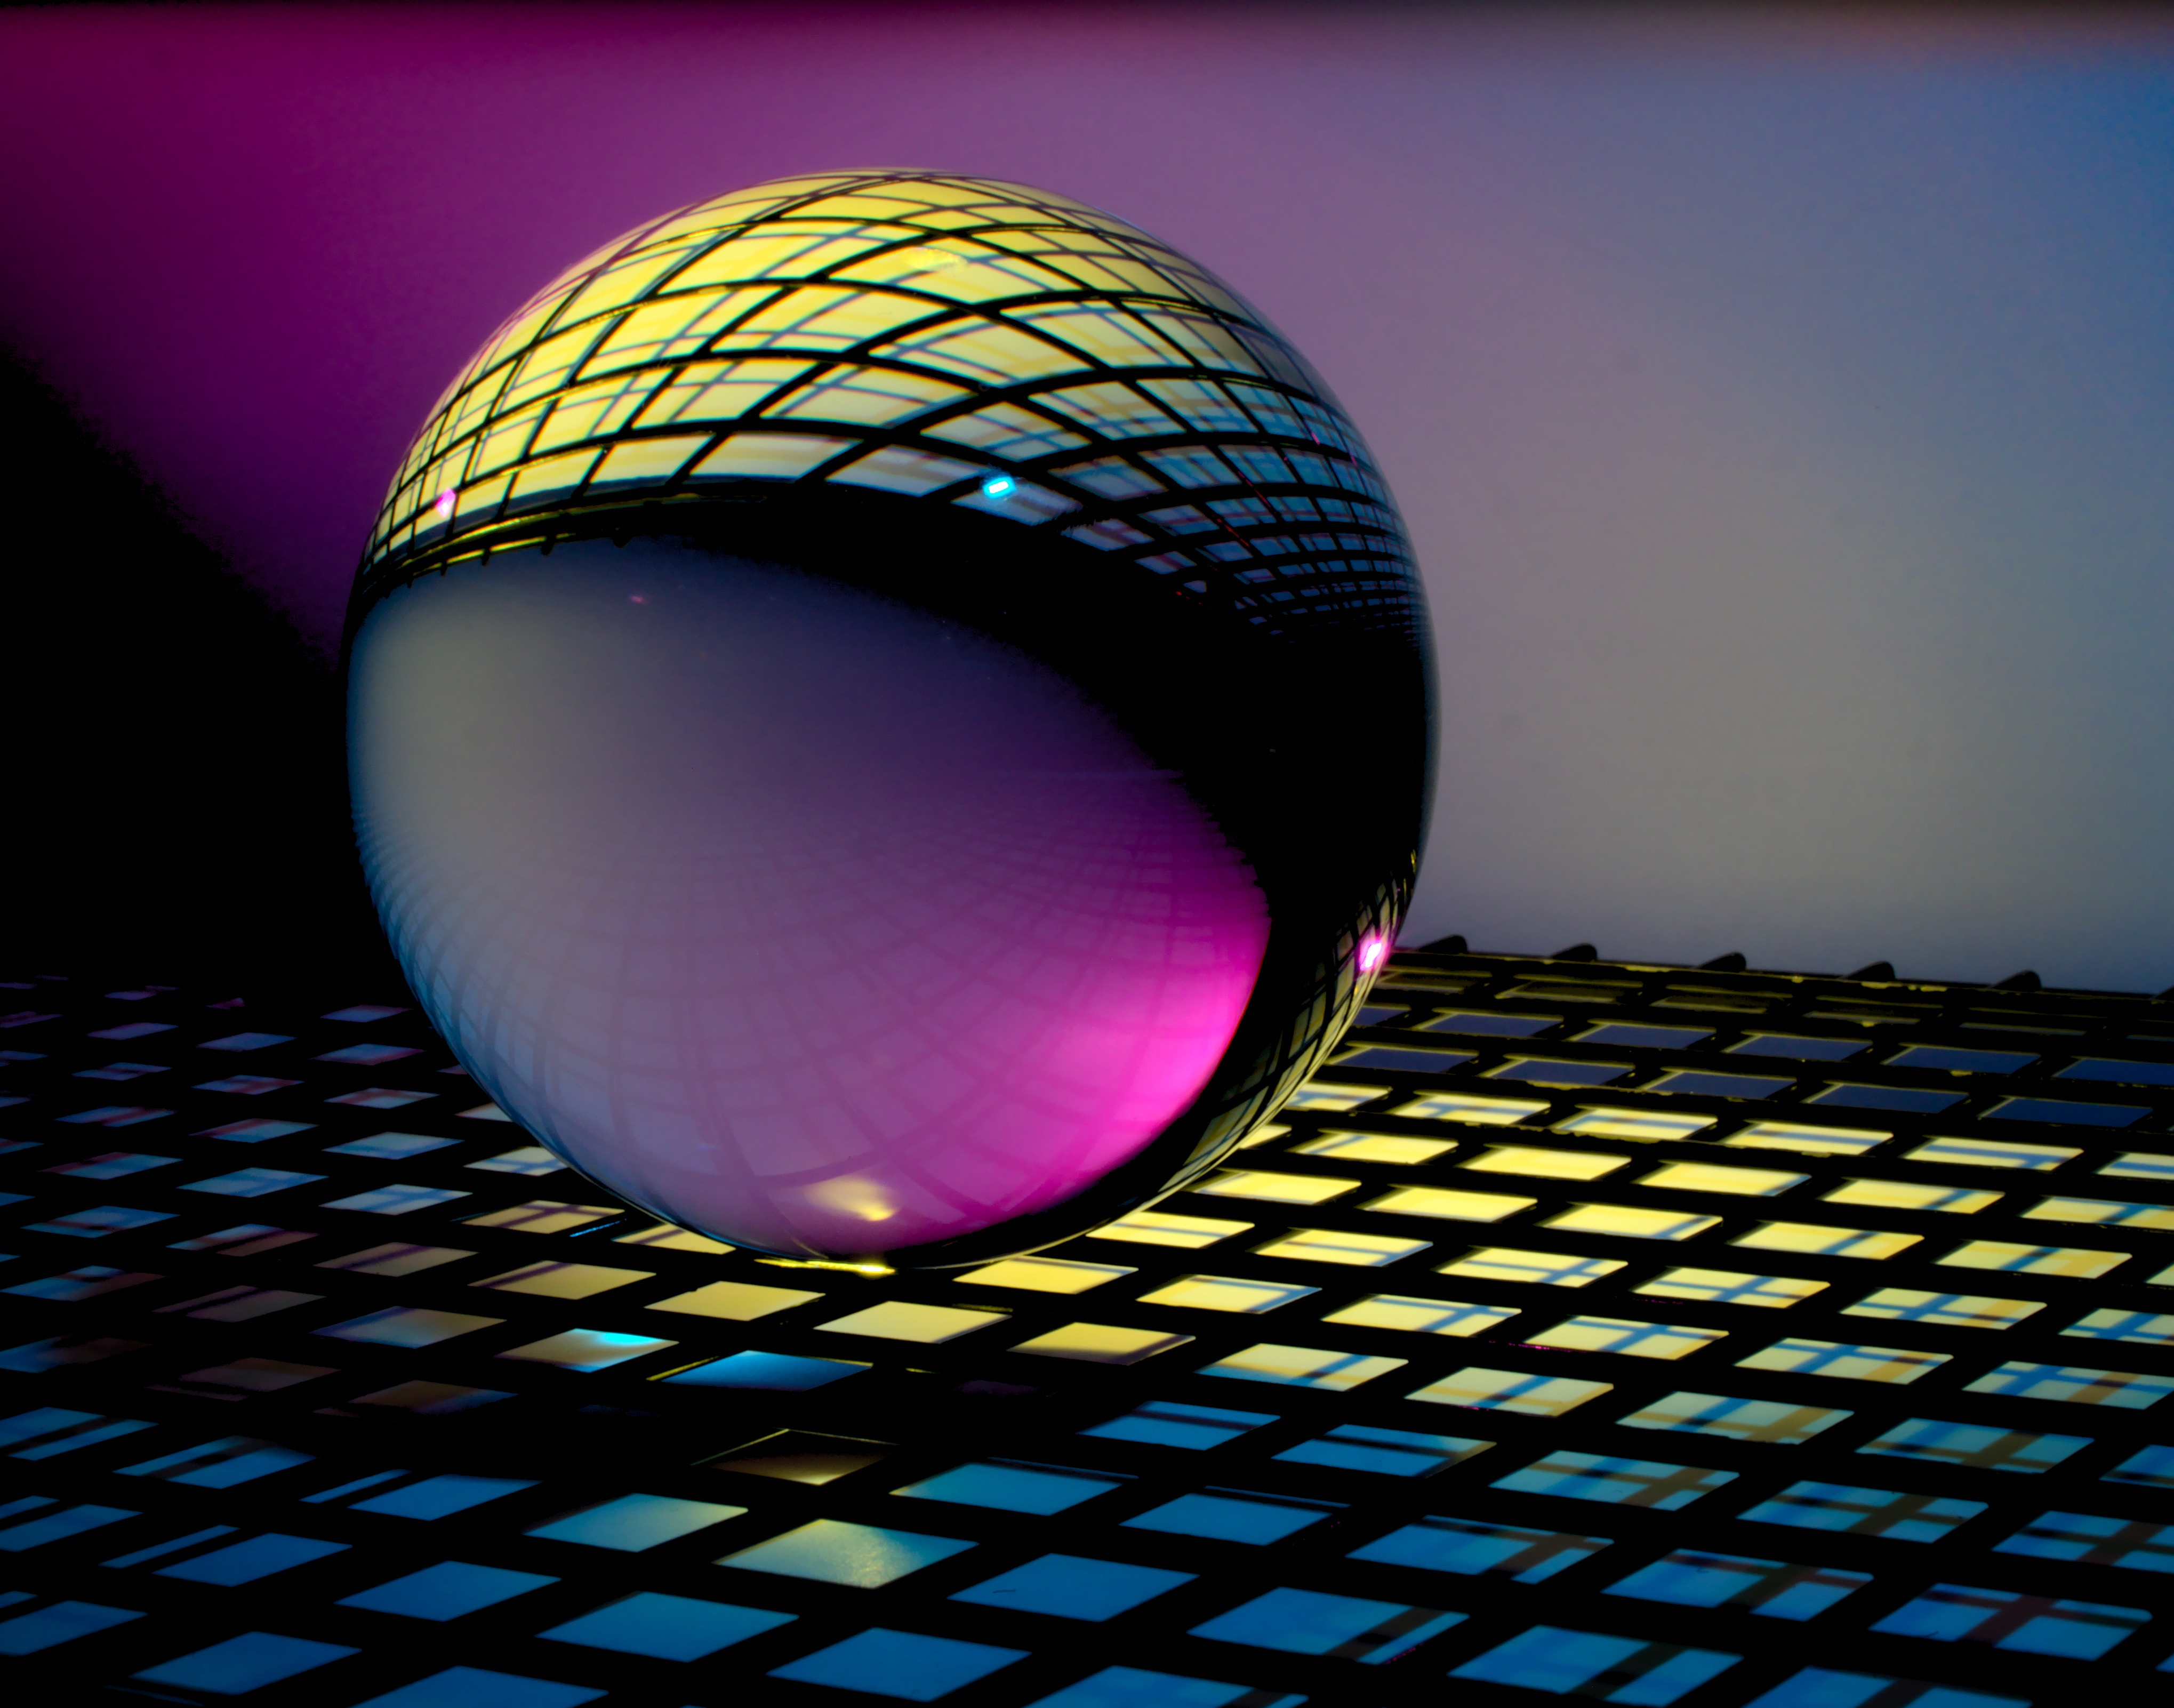
\includegraphics[width=10cm]{michael-dziedzic-qDG7XKJLKbs-unsplash.jpg}
    % \caption{Caption}
    \label{fig:enter-label}
\end{figure}



\clearpage

  % \textsf{黑体\textbf{加粗}}


\section*{题目}


\textbf{Step 1 简要综合行研}
\begin{enumerate}
    \item  整合信息得到一个相对简答的AGI行研报告。
    \item   自主学习并选择一个逻辑去表达你的AGI行业研究成果。
    \begin{enumerate}
        \item 包含中国及北美各自的行业格局的分析。
        \item 选择该逻辑组织信息的原因。
        \item 得到至少3个行研得到的洞见。
    \end{enumerate}
\end{enumerate}

% 1. 整合信息得到一个相对简答的AGI行研报告。
% 2. 自主学习并选择一个逻辑去表达你的AGI行业研究成果。
% 2.1 包含中国及北美各自的行业格局的分析。
% 2.2 选择该逻辑组织信息的原因。
% 2.3 得到至少3个行研得到的洞见。
\textbf{Step 2 模拟决策}
\begin{enumerate}
    \item 假设有1000万资金,基于Step 1形成一个投资策略。
    \begin{enumerate}
        \item  二级市场投资占比<=20\%, 标注理由。
        \item  一级市场股权投资或者孵化策略<=100\%。
        \item  解释一级市场股权投资的细分赛道和下注方式。
        \item 如上策略不需要考虑实际操作难度和成本。
    \end{enumerate}
    \item 条件不变,资金变为1亿元人民币。
\end{enumerate}

\textbf{Step 3 信息趣味}

\begin{enumerate}
    \item  如果可以和Sam Altman等AGI领域的人交流,最想问的5个问题?
    \item 推荐最受益的信息源,包括最看好的VC、最欣赏的从业者,每个不超过5个。并阐释理由。
\end{enumerate}

\textbf{Step 4 信息推送}

模拟一天的推送信息,格式和形式不限。
\newpage
\section{简要AGI综合行研}
*注:因为大模型是迈向AGI目前为止可行性最高的实现路径,因此以下分析和研究均围绕大模型或者基于大模型的多模态模型展开。
\subsection{大模型发展标志性事件梳理}
\begin{enumerate}
    \item 2015年,OpenAI成立。
    \item 2017年,Google推出Transformer模型,参数量首次达到上亿规模。
    \item 2018年,Google推出Bert模型,参数量达到3亿规模;OpenAI推出GPT。
    \item 2019年,OpenAI推出GPT-2模型,参数量达到15亿规模。
    \item 2020年,OpenAI推出GPT-3模型,参数量达到1750亿;微软和英伟达发布MT-NLG模型,参数量达到5300亿。
    \item 2021年,Google发布Switch Transformer模型,参数量达到1.6万亿。
    \item 2022年,OpenAI推出基于GPT-3.5的ChatGPT,成为现象级产品。
    \item 2023年,OpenAI推出GPT-4,参数规模和细节尚未公开。
\end{enumerate}
大(语言)模型作为人类在人工智能领域最先进的产出,同时也是最接近实现AGI的产品,其发展极其迅速。并且有进一步加速的趋势。
\subsection{大模型时代下的核心竞争力}
\begin{enumerate}
    \item 算法
    \item 数据
    \item 算力
\end{enumerate}
算法或者模型本身,本质是其相关的研发实力,(同时也是在AGI领域科技树的某个技术分支的押注)是一个公司的最强的壁垒和发展护城河。越先进的模型,越可能打造出优质的产品,才能吸引到广大消费者群体和后续的商业化,因此算法是做AGI公司的核心竞争力。

数据是训练的基础,训练数据质量的好坏、范围直接影响模型训练的结果,从这点来看,模型决定了效果的上限,但是数据决定了效果的实际完成度。当数据和模型都配套好才可以发挥模型的最好的效果。

算力是发展大模型的前提。在当前的模型参数下,没有庞大算力的公司意味着可能直接错失进入AGI行业的入场券,这也意味着当前AGI行业只能是算力充足、资金雄厚、研发实力强劲的巨头可以参与。同时因为NVIDA的A100销售禁令,可能会造成国内算力缺口。

\subsection{中国和北美大模型竞争格局}
首先需要理清一个逻辑是:不是领先的大模型占据高端市场,落后一些的大模型占据低端市场,而是领先的大模型几乎会占领一切市场。和传统的高端——中端——低端市场有与之相对应的高端——中端——低端消费群体不同,民用大模型的使用成本已经降低到一个较低的水平(按照GPT-4的订阅费用来衡量),因此高端中端低端用户都可以消费起行业最领先的模型和产品,同时因为行业头部的模型(GPT-4)的使用体验要远大于中部的模型(百度的文心一言、阿里的通义千问等国产大模型),会导致各个市场的用户会集中使用最好的模型(除非有不可抗因素,如IP禁用、大陆地区封号等等)。

因此这对于中国发展大模型是有严重劣势的,因为国产大模型可能和北美有1-2代的版本代差,而这个追赶期目前仍不确定。\textit{“李彦宏称自己前段时间接受采访时说跟ChatGPT的差距大约是两个月,有点断章取义,因为自己后面紧接着说:‘这不是重点,重点是这两个月的差距我们要用多长时间才能赶上,也许很快,也许永远也赶不上。’”}

我们从“大模型时代下的核心竞争力”梳理的三个角度来进行分析。

\noindent\textbf{模型:}
\begin{itemize}
    \item 北美有顶流——OpenAI的GPT-4及GPT-3.5,号称ChatGPT的最强竞品——anthropic的Claude,传统AI巨头Meta的LLaMA,Amazon的Amazon Titan等等。
    \item 国内有百度的文心一言、阿里的通义千问、华为的盘古、科大讯飞的星火认知大模型、商汤的SenseChat、360智脑、腾讯的混元等。
\end{itemize}
由于大部分均仍在内测阶段,无法对其进行完整的测试。但是根据一份来源于真格基金的测评来看,国内最强的模型是百度的通义千问,综合表现较好的商汤的SenseChat。但是仍然不及ChatGPT-3.5。从直接的测试结果来看,国内最好的模型效果是ChatGPT-3.5的75\%左右。


\noindent\textbf{数据:}
从中文语料库和英文语料库来看,都应该是足够训练大模型的,但是国内的数据标注产业可能相较于北美较为落后。

\noindent\textbf{算力:}
算力问题可能是国内最明显的短板,最主要的原因就在于Nvida的A100禁令,国内有超大规模算力(1万块A100规模)的公司屈指可数。

\subsection{洞见}
\begin{enumerate}
    \item 整体来看,大模型产业北美从各个方面都处于领先地位,国产大模型在追赶,但是处于一个十分危险的境地(好在有Great firewall)。这次的AGI竞赛可能会直接关系到一些互联网科技公司的生死存亡。
    \item 国内有可能的发展是数据标注行业,虽然相对北美较为弱势,但是行业门槛较低,如果发挥一定人力成本优势,或许存在发展空间。
    \item 比较看好的是百度和华为的模型,因为具有先发优势,同时两家都在AI领域也有积累。其次是字节的模型,字节在AI领域的积累也比较深厚,但是由于发展时间较晚,可能还存在一定的落地期。
    \item 在这种情况下,大厂可能需要两条腿走路——既要发展自己的大模型,又要积极支持和收购在技术路线上有正确探索的中小公司。
    \item 在GPT部署使用场景下,云服务和向量数据库可能会更大规模使用,需要关注有相关业务的公司。
\end{enumerate}


\newpage
\section{Step 2 模拟决策}
\subsection{1000万人民币筹码的投资策略}
1000万的资金按照2:8的二级市场投资和一级市场投资划分。
个人的建议如下:
\begin{enumerate}
    \item 200万中按照4:2:2:1:1的比例分别投资Nvida、Microsoft、Google、Amazon、百度股票。
    \item 800万中投资3-4家做\textbf{数据标注}的Startup的天使轮。*如果有可能,投资1-2个\textbf{非常规半导体算力}的Startup天使轮。或者一些做\textbf{向量数据库}的Startup天使轮。前提是技术路线可落地、前景好、靠谱等。
\end{enumerate}

\subsection{1亿元人民币筹码的投资策略}
相较于1000万筹码,1亿元可以到达给几个小型公司A——B轮融资的程度。
但是个人认为,和1000万人民币级别的投资策略不会有太大区别。因为可投资的范围(一级市场)到不了做算力、模型的公司上。
可能到20亿人民币规模会存在一些明显的改善,因为当前做的一些比较优秀的公司估值普遍在20亿美元以上。\textit{2023年3月9日Anthropic筹资11亿美元,投资者包括谷歌、Skype联合创始人Jaan Tallinn和FTX前首席执行官Sam Bankman-Fried等。}
因此对于1亿人民币规模的筹码而言,个人的建议如下:
\begin{enumerate}
    \item 20\%资金按照4:2:2:1:1的比例分别投资Nvida、Microsoft、Google、Amazon、百度股票。
    \item 80\%资金投资3-4家做\textbf{数据标注}的Startup的A轮。*如果有可能,投资1-2个\textbf{非常规半导体算力}的Startup的A轮。或者1-2个做\textbf{向量数据库}的Startup的A轮。前提是技术已经有一定落地,发展成本可控、前景较为明确,靠谱等。
\end{enumerate}














\newpage
\section{信息趣味}
\subsection{向AGI领域相关人员提问}
\begin{enumerate}
    \item openAI的GPT如何解决用户隐私数据安全?(向Sam Altman)
    \item 您真的认为AGI会失控吗?如果是的话,人类为什么控制不了它呢?(向Elon Musk)
    \item 您曾否定了自回归模型,那您是如何看待GPT-4的成果和括“涌现”现象的发生呢?(向Yann LeCun)
    \item 您觉得您和OpenAI相比,百度在技术领域最大的优势是什么?(向李彦宏)
    \item 国内互联网公司其实较早都布局了大模型,但是字节今年才成立相关研究团队,明显慢于同行,您觉得其中的原因是什么呢?(向Liang Rubo)
\end{enumerate}

\subsection{推荐的信息源}
\begin{itemize}
    \item 最好的信息源:Github Daily Trending下的源代码。(“Don’t talk,show me your code”)
    \item 最看好的VC机构:YC (最著名、最成功的创业孵化机构之一)、红杉资本(最著名的、最成功的VC之一)。无看好的本土VC。
    \item 最欣赏的从业者:Sam Altman(OpenAI创始人,没有股权,因为热爱从事AI)、Yann LeCun(图灵奖获得者,在有充分理由的前提下否认自回归模型,提出“世界模型”架构)
\end{itemize}
\newpage
\section{信息推送}

\begin{figure}[htpb]
    \centering
    \includegraphics[width=15cm]{noname-2.png}
    % \caption{Intro}
    \label{fig:enter-label}
\end{figure}


\noindent\textbf{The Revolution in Large Language Models: A Pivotal Moment in Our Quest Towards Artificial General Intelligence}

\subsection{Introduction}

The quest to design and develop Artificial General Intelligence (AGI) has seen numerous significant breakthroughs, with each phase of technological advancement bringing us a step closer to this pinnacle of AI. The current revolution in large language models like OpenAI's GPT-3, however, stands out as a unique turning point in this journey. Unlike previous advancements, this revolution exhibits superior capabilities, including the understanding of context, generation of creative content, and the ability to learn from fewer examples, thus bringing us the closest yet to AGI.

\subsection{Understanding Context}

One of the key differences that make this revolution different from the ones before is the ability of large language models to understand context. Previous AI models were significantly limited in their understanding of human language due to their inability to comprehend context. They could process keywords and syntax but struggled with idioms, metaphors, and expressions that required contextual interpretation. 

Modern large language models, however, are trained on vast volumes of text data from the internet, enabling them to infer the meaning from context and generate responses that are contextually accurate. This contextual understanding goes beyond simple keyword recognition, bringing us closer to AGI, which would possess the ability to understand and interact with its environment in a way that is indistinguishable from human beings.

\subsection{Generative Capabilities and Creativity}

Another distinguishing feature of the current revolution in large language models is their generative capabilities. Earlier AI models were predominantly task-specific, designed to perform specific tasks within strict parameters. They lacked the capability to generate creative solutions or produce unique content.

In contrast, large language models can generate coherent and contextually appropriate content, whether it be completing a story, writing an essay, or even composing poetry. This ability to generate creative output is a significant step towards AGI, which would be expected to exhibit creativity and innovation, traits currently unique to human intelligence.

\subsection{Learning from Fewer Examples}

The current revolution in large language models also represents a significant leap in the efficiency of learning. Previous models required vast amounts of training data and explicit instructions to learn a new task. This was time-consuming and often led to models that were excellent at one specific task but useless outside of it.

In contrast, large language models can learn from fewer examples, often requiring only a few instances of a task to understand it. This ability to learn efficiently and generalize from few examples brings us significantly closer to AGI, which would be expected to learn and adapt to new tasks and environments with minimal instruction, much like a human being.

\subsection{Conclusion}

The current revolution in large language models signifies a significant leap in our pursuit of AGI. By understanding context, generating creative content, and learning from fewer examples, these models have taken us closer than ever to achieving AGI. However, it is essential to bear in mind that while we are closer than ever, we are not there yet. There are still significant challenges to overcome, such as imbuing AI with common sense understanding and the ability to form meaningful relationships between different knowledge domains. Nevertheless, the progress made with large language models is an encouraging sign of what the future may hold.


\end{document}
